\documentclass[12pt]{article}
\usepackage{amsmath}
\usepackage[utf8]{inputenc}
\usepackage{natbib}
\bibliographystyle{abbrvnat}
\setcitestyle{authoryear,open={((},close={))}}
\usepackage{graphicx}
\usepackage{float}
\usepackage[margin=1in]{geometry}
\usepackage{fancyhdr}
\usepackage[framed,numbered,autolinebreaks,useliterate]{mcode}

\pagestyle{headings}
\fancyhf{}
\rhead{Max Le 901223283}
\lhead{MTH5315 FINAL EXAM}

\title{MAE 5315 NUMERICAL METHODS FOR PDE \\ FINAL EXAM}
\date{\today}
\author{\Huge Max L$\hat{\textrm{e}}$ \\ \\ ID: 901223283}
\begin{document}
	\maketitle
	\newpage
	\tableofcontents
	\newpage
	\listoffigures
	\newpage
	\section{INTRODUCTION}
	\subsection{Problem Statement}
	In this problem, we are required to solve a 2D heat conduction equation:		
	\begin{equation}
		u_t = u_{xx} + u_{yy} + f(x,y,t)
	\end{equation}
	on the domain $x\in [0,1]$ and $y\in [0,1]$ with the source function defined as: 
	
	\begin{equation}
	f(x,y,t) = e^{-t}sin(\pi x)sin(\pi y)(2\pi ^2 -1)
	\end{equation}	
	The solution is 0 on the boundary, in other words: 
	\begin{align*}
		u(0,y,t) &= u(1,y,t) = 0 \\ 
		u(x,0,t) &= u(x,1,t) = 0
	\end{align*}  	
	The initial condition is given as follow: 
	\begin{equation}
	u(x,y,0) = sin(\pi x)sin(\pi y)
	\end{equation}
	We are required to solve the PDE using the Alternate Direction Implicit (ADI) scheme using a $dx = 1/64$ and up to t = 1.0  

	\subsection{Analytical Solution}
	At first, the analytical solution is calculated. We start with a homogeneous PDE (f(x,y,t) = 0) and assume the solution $u(x,y,t) = X(x)Y(y)T(t)$, and substitute into the PDE, we get the following system of eigenvalue problems. 
	
	\begin{equation*}
		\dfrac{T'(t)}{T(t)} = \dfrac{X'(x)}{X(x)} + \dfrac{Y'(y)}{Y(y)} = -\lambda
	\end{equation*}
	The sum between X and Y can also be decomposed into a sub-eigenvalue problems, we will call this $-\mu$. Putting together, we have:
	\begin{align*}
		T'(t) + \lambda T = 0 \text{ where } T(0) = f(x,y,0)\\
		Y"(y) + \mu Y(y) = 0 \text{ where } Y(0) = Y(1) = 0 \\
		X"(x) + (\lambda - \mu) X(x) = 0 \text{ where } X(0) = X(1) = 0
	\end{align*}
	Solving the Y equation first, for the case when $\lambda = 0$:
	\begin{align*}
		Y(y) = C1 + C2y
	\end{align*}
	Substituting the boundary conditions for Y will yield both C1 = C2 = 0, which is a trivial solution and we do not want this.
	Now for the case when $\lambda = m^2 > 0$: 
	\begin{align*}
		Y(y) = C1cos(my) + C2sin(my)
	\end{align*}
	Again, plugging in the boundary conditions for Y yield C1 = 0; but this time we have the option of not allowing C2 to be 0. This implies m = k$\pi$, for k = 1,2... Therefore, the first eigenvalue is known and the equation for Y is: 
	\begin{align*}
		Y(y) = sin(m\pi y), m = 1,2,..
	\end{align*}
	Substitute $\lambda$ into the X equation, we can follow the similar procedure and get the solution as follow: 
	\begin{align*}
		X(x) = sin(n\pi x), n = 1,2,..
	\end{align*}
	Then our general solution will look like this: 
	\begin{align*}
		u(x,y,t) = \sum_{n=1}^{\infty}\sum_{m=1}^{\infty} sin(n\pi x)sin(m\pi y)B_{mn}(t)
	\end{align*}
	Next, we expand the source function, f(x,y,t), into a Fourier series and compare
	\begin{align*}
		f(x,y,t) &= e^{-t}sin(\pi x)sin(\pi y)(2\pi ^2 -1)\\
		&= \sum_{n=1}^{\infty}\sum_{m=1}^{\infty}F_{mn}(t)sin(n\pi x)sin(m\pi y)
	\end{align*}
	We note that: when m = n = 1 $=> F_{mn}(t) = e^{-t}(2\pi ^2 -1)$. Else, $F_{mn}(t) = 0$. Now, we use the general solution in the form of the Fourier series and get $u_t, u_xx, u_yy$ by taking derivatives. This yields the following: 
	\begin{align*}
		u_t(x,y,t) &= \sum_{n=1}^{\infty}\sum_{m=1}^{\infty} sin(n\pi x)sin(m\pi y)B'_{mn}(t)\\
		u_{xx}(x,y,t) &= -\sum_{n=1}^{\infty}\sum_{m=1}^{\infty} (n^2 \pi^2)sin(n\pi x)sin(m\pi y)B_{mn}(t)\\
		u_{yy}(x,y,t) &= -\sum_{n=1}^{\infty}\sum_{m=1}^{\infty} (m^2 \pi^2)sin(n\pi x)sin(m\pi y)B_{mn}(t)
	\end{align*}
	Equating these along with the Fourier expansion of the source term into the original PDE, doing calculation for each n and m, and simplifying, we get a first order ODE. 
	\begin{align*}
		B'_{mn}(t) = -(m^2+n^2)\pi ^2B_{mn}(t) + F_{mn}(t)
	\end{align*}
	For values of $m \neq n \neq 1, B_{mn}(t) = 0$ because: we will not be able to get the initial condition $u(x,y,0) = sin(\pi x)sin(\pi y)$.  Therefore, for different values of m, n: $B_{mn}(t) = 0$ and from before: $F_{mn}(t) = 0$. The only value left is m = n = 1, this gives us the following ODE:
	
	\begin{equation}
		B'_{11}(t) = -(2\pi^2)B_{11}(t) + e^{-t}(2\pi ^2 -1)
	\end{equation}
	Using the integration factor method, we can solve this equation as follow, dropping subscript 11:
	
	\begin{align*}
		e^{2\pi^2 t}B'(t) + e^{2\pi^2 t}B(t)(2\pi ^2) &= e^{(2\pi^2 -1)-1}(2\pi ^2 -1)\\
		\int\limits_{0}^{t} \dfrac{d}{dt}\left(Be^{2\pi^2 t}\right) dt &= \int\limits_{0}^{t}e^{(2\pi^2 -1)-1}(2\pi ^2 -1)\\
		\boxed{B(t)= e^{-t}}
	\end{align*}
	Substitute this into the general form of the solution, we get the following exact solution:
	
	\begin{equation}
		\boxed{u(x,y,t) = e^{-t}sin(\pi x)sin(\pi y)}
	\end{equation}
		
	\subsection{Numerical Solution}
	For our numerical solution, the basic idea is to apply a second order central difference discretization like this:
	
	\begin{equation}
		u_i = \dfrac{u_{i+1} - 2u_i + u_{i-1}}{\Delta x^2} + O(\Delta x^2)
	\end{equation}
	
	
	The stencil used in this problem is a node centered grid, the spacing, $\Delta x = \Delta y$, is used.	
	
	\begin{figure}[H]
		\hfill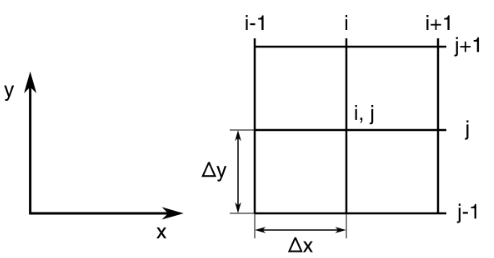
\includegraphics[width=80mm,height= 40mm]{stencil.png}\hspace*{\fill}
		\caption{Numerical stencil}
	\end{figure}
	\noindent
	Let $U_{ij}^n$ be the numerical solution at location (i,j) at time n. For the ADI scheme, we apply second order central difference discretization to advance solution from n to n+1/2:
	
	\begin{equation}
		\dfrac{U_{ij}^{n+1/2}-U_{ij}^{n}}{\Delta t/2} = \left[ \dfrac{U_{i+1,j}^{n+1/2}-2U_{ij}^{n+1/2} + U_{i-1,j}^{n+1/2}}{\Delta x^2}      +    \dfrac{U_{i,j+1}^{n}-2U_{ij}^{n} + U_{i,j-1}^{n}}{\Delta y^2}                 \right] + f_ij^{n+1/4}
	\end{equation}
	Then, the solution obtained at n+1/2 is then used to advance to final solution at time n+1. 
	
	\begin{equation}
		\dfrac{U_{ij}^{n+1}-U_{ij}^{n+1/2}}{\Delta t/2} = \left[ \dfrac{U_{i+1,j}^{n+1/2}-2U_{ij}^{n+1/2} + U_{i-1,j}^{n+1/2}}{\Delta x^2}      +    \dfrac{U_{i,j+1}^{n+1}-2U_{ij}^{n+1} + U_{i,j-1}^{n+1}}{\Delta y^2}                 \right] + f_{ij}^{n+3/4}
	\end{equation}
	Both equation 6 and 7, when written out, will result in a tri-diagonal system. Rewriting the systems (putting everything we know at time n to the right hand side), and denoting the diffusion number as: $D_x = \dfrac{\alpha\Delta t}{\Delta x^2}$ and $D_y = \dfrac{\alpha\Delta t}{\Delta y^2}$, we get: 
	
	\begin{equation}
		(1+D_x)U_{ij}^{n+1/2} + \left(\dfrac{D_x}{2}U_{i+1,j}^{n+1/2}\right) +\left(\dfrac{D_x}{2}\right)U_{i-1,j}^{n+1/2} =  (1+D_y)U_{ij}^{n} + \left(\dfrac{D_x}{2}U_{i,j+1}^{n}\right) +\left(\dfrac{D_y}{2}\right)U_{i,j-1}^{n}+\dfrac{\Delta t}{2}f_ij^{n+1/4}  
	\end{equation}
	
	\begin{equation}
	(1+D_y)U_{ij}^{n+1} + \left(\dfrac{D_y}{2}U_{i,j+1}^{n+1}\right) +\left(\dfrac{D_y}{2}\right)U_{i,j-1}^{n+1}  = (1+D_x)U_{ij}^{n+1/2} + \left(\dfrac{D_x}{2}U_{i+1,j}^{n+1/2}\right) +\left(\dfrac{D_x}{2}\right)U_{i-1,j}^{n+1/2} + \dfrac{\Delta t}{2}f_{ij}^{n+3/4}
	\end{equation}
	The tri-diagonal system looks like this: 

	\begin{figure}[H]

	\[
	\begin{bmatrix}
	(1-D_x) & (D_x/2) & 0 & \dots & 0 \\
	(D_x/2) & (1-D_x) & (D_x/2) & \dots & 0 \\
	0 & (D_x/2) & (1-D_x) & (D_x/2) & \dots \\
	\dots  & \dots  & \dots  & \dots & \dots  \\
	\dots & \dots & \dots & \dots & \dots 
	\end{bmatrix}
	\begin{bmatrix}
	u^{n+1/2}_1 \\ u^{n+1/2}_2 \\ u^{n+1/2}_3 \\ \dots \\ u^{n+1/2}_n 
	\end{bmatrix}
	=
	\begin{bmatrix}
	f^n_1 \\ f^n_2 \\ f^n_3 \\ \dots \\ f^n_n 
	\end{bmatrix}
	\]

	\caption{X sweep tridiagonal system}

	\end{figure}



	\begin{figure}[H]

	\[	
	\begin{bmatrix}
		(1-D_y) & (D_y/2) & 0 & \dots & 0 \\
		(D_y/2) & (1-D_y) & (D_y/2) & \dots & 0 \\
		0 & (D_y/2) & (1-D_y) & (D_y/2) & \dots \\
		\dots  & \dots  & \dots  & \dots & \dots  \\
		\dots & \dots & \dots & \dots & \dots 
	\end{bmatrix}
	\begin{bmatrix}
		u_1^{n+1} \\ u_2^{n+1} \\ u_3^{n+1} \\ \dots \\ u_n^{n+1} 
	\end{bmatrix}
	=
	\begin{bmatrix}
		f^{n+1/2}_1 \\ f^{n+1/2}_2 \\ f^{n+1/2}_3 \\ \dots \\ f^{n+1/2}_n 
	\end{bmatrix}
	\]
	\caption{Y sweep tridiagonal system}
	\end{figure}
	\noindent	
	where f1,..,fn denote the known value at each node, and the superscript denotes the time level (n,n+1/2, or n+1). The right hand side is evaluated at each time step and at each node. In order to solve this system efficiently, we use Thomas Algorithm. 
	
	\subsection{Thomas Algorithm Overview}
	Denoting the diagonal of the matrix as b,the subdiagonal as a and the superdiagonal as c, the solution vector as u and the right hand side vector as d, we can do the following: 
	  
	
	\begin{figure}[H]
		
		\[	
		\begin{bmatrix}
		b1 & c1 & 0 & \dots & 0 \\
		a1 & b2 & c2 & \dots & 0 \\
		0 & a2 & b3 & c3 & \dots \\
		\dots  & \dots  & \dots  & \dots & \dots  \\
		\dots & \dots & \dots & \dots & \dots 
		\end{bmatrix}
		\begin{bmatrix}
		u_1 \\ u_2 \\ u_3 \\ \dots \\ u_n 
		\end{bmatrix}
		=
		\begin{bmatrix}
		d_1 \\ d_2 \\ d_3 \\ \dots \\ d_n 
		\end{bmatrix}
		\]
		\caption{Thomas parameters matrix}
	\end{figure}
	\noindent
	The ith equation in the sytem may be written as:	
	\begin{align*}
		a_iu_{i-1} + b_iu_i+ c_iu_{i+1} = d_i
	\end{align*}
	where $a_1$ = 0 and $c_n$ = 0. Looking at the system of equations, we see that ith unknown can be expressed as in terms of the (i+1)th unknown: 	
	\begin{align*}
		u_i &= P_iU_{i+1}+Q_i\\
		u_{i-1}&=P_{i-1}iU_i+Q_{i-1}
	\end{align*}  
	If the all equations are written out like this, then the coefficient matrix would form an upper triangular matrix. Plugging these equations into the ith equation of the tri-diagonal matrix, we get the following expressions for P and Q: 
	\begin{align*}
		P_i &= \dfrac{-c_i}{b_i+a_iP_{i-1}}\\
		Q_i &= \dfrac{d_i-a_iQ_{i-1}}{b_i+a_iP_{i-1}}
	\end{align*} 
	These recursive relations show that ith unknown can be calculated when i-1 unknown is available. At i = 1, we have: 
	\begin{align*}
		P_1 &= \dfrac{-c1}{d1}\\
		Q_1 &= \dfrac{d1}{b1}
	\end{align*}
	Below is a Fortran implementation for this algorithm, for our case, this will coded in Matlab. 
	
	
	\begin{figure}[H]
		\hfill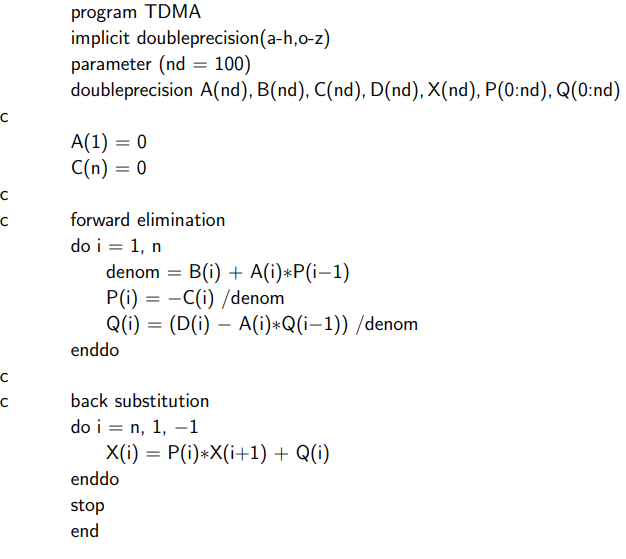
\includegraphics[width=150mm,height= 100mm]{thomaspseudo.png}\hspace*{\fill}
		\caption{Thomas Algorithm in Fortran}
	\end{figure}
	The basic idea for this ADI algorithm is to do: 
	\begin{enumerate}
		\item X sweep
		\begin{itemize}
			\item Use solution at n to solve X implicitly using and Y explicitly
			\item Obtain solution at n+1/2
		\end{itemize}
		\item Y sweep
		\begin{itemize}		
			\item Use solution at n+1/2 to solve X implicitly using and Y explicitly
			\item Obtain solution at n+1
		\end{itemize}
		\item Repeat until reach a specified time.
			
	\end{enumerate}

	\newpage	
	\section{RESULTS}
	Below are the results obtained from this method: 
	\subsection{Analytical and Numerical Results}
	\begin{figure}[H]
		\hfill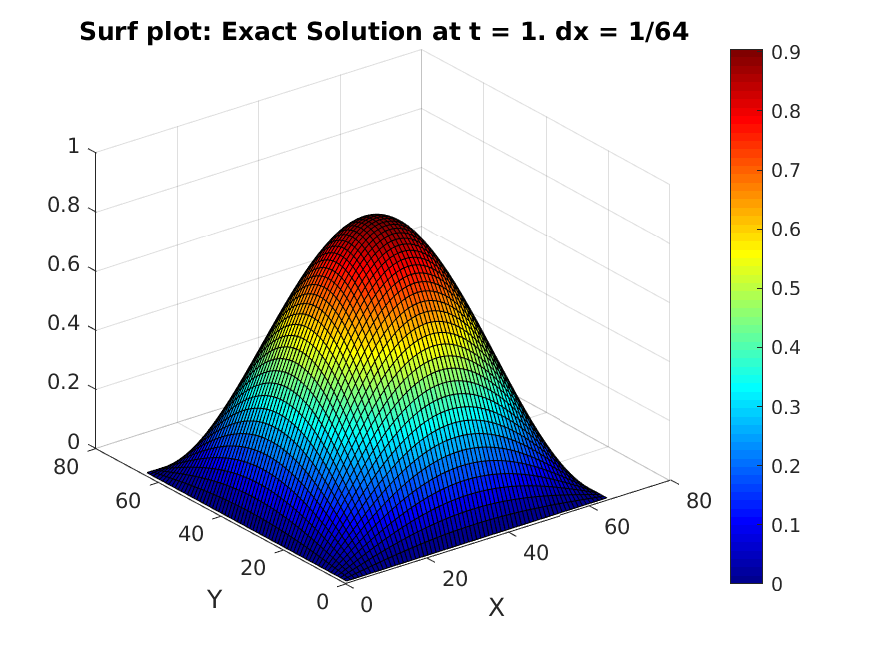
\includegraphics[width=150mm,height= 100mm]{exactsurf.png}\hspace*{\fill}
		\caption{Analytical solution 3D plot}
	\end{figure}

	\begin{figure}[H]
		\hfill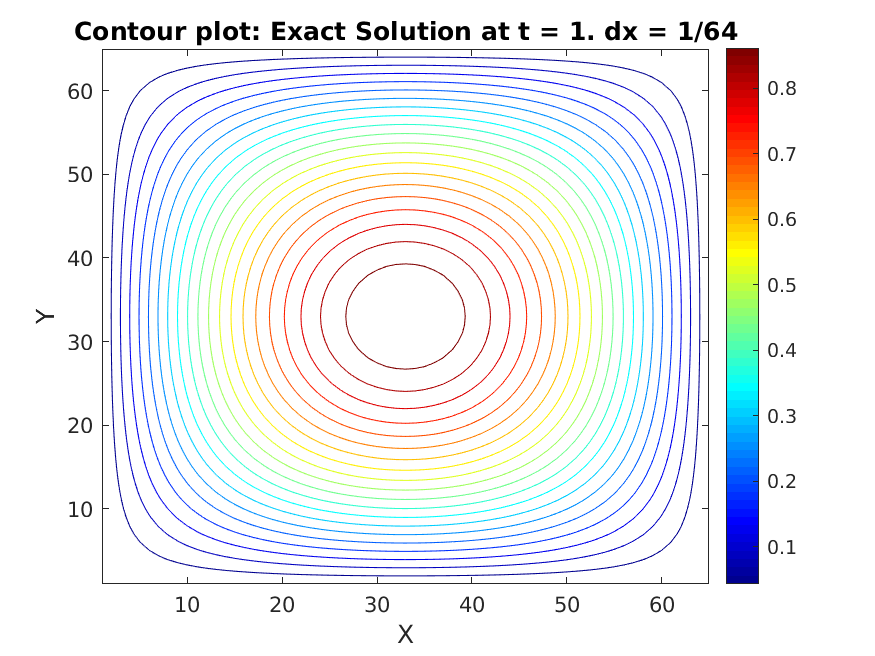
\includegraphics[width=150mm,height= 100mm]{exactcontour.png}\hspace*{\fill}
		\caption{Analytical solution 2D plot}
	\end{figure}

	\begin{figure}[H]
		\hfill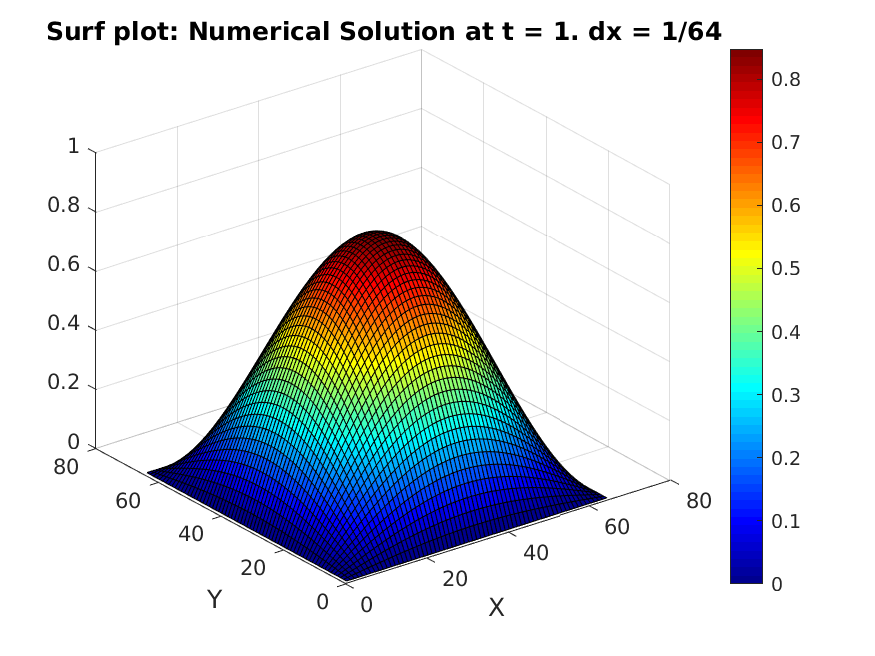
\includegraphics[width=150mm,height= 100mm]{numsurf.png}\hspace*{\fill}
		\caption{Numerical solution 3D plot}
	\end{figure}
	
	\begin{figure}[H]
		\hfill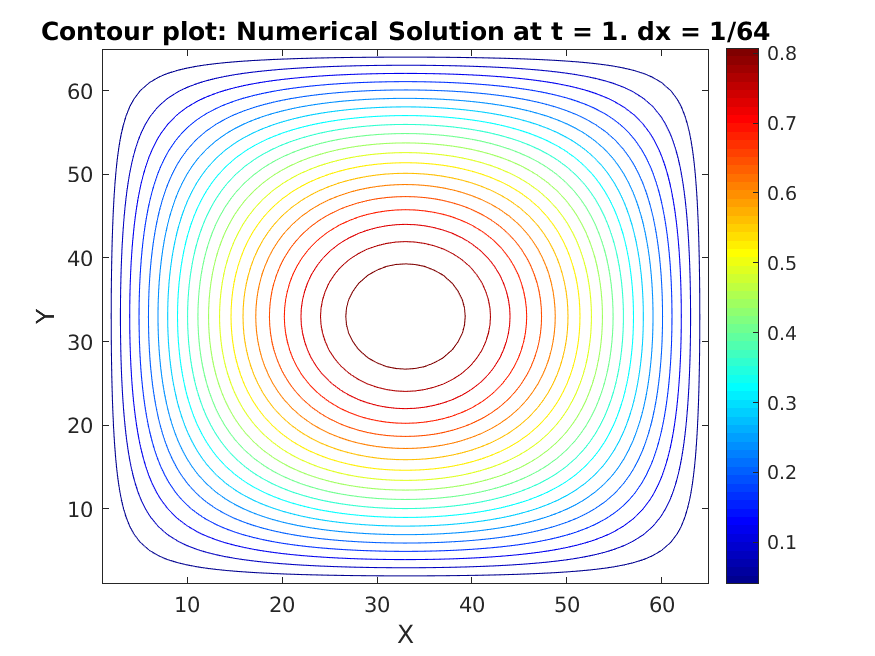
\includegraphics[width=150mm,height= 100mm]{numcontour.png}\hspace*{\fill}
		\caption{Numerical solution 2D plot}
	\end{figure}
	\noindent
	We can see that the numerical result is very close to the analytical one. At first glance, both solutions have the same shape. We can still very clearly the tip of the cone. Although, the colorbar shows that the maximum point at the tip is slightly off (0.9 for analytical vs 0.8 for numerical to 2 decimal places). Our original problem is a 2D heat conduction equation whose source term is controlled via a sinusoidal ($	f(x,y,t) = e^{-t}sin(\pi x)sin(\pi y)(2\pi ^2 -1)$); therefore, the end result is also a sinusoidal, but because of superposition principle, we have a sinusoidal in 3D.

	\subsection{Error and Convergence Analysis}
	
	 In other to investigate the error and convergence, we first need to plot to see how far away from the analytical solution is the numerical solution. To do that, we subtract the numerical from the analytical and then plot the error. 
	 \begin{figure}[H]
	 	\hfill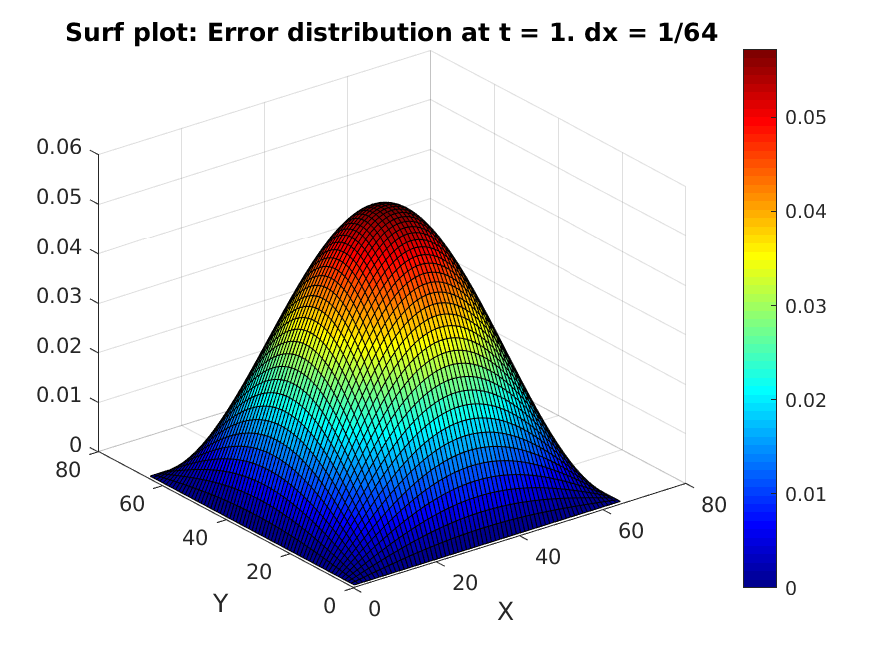
\includegraphics[width=150mm,height= 90mm]{surf_error.png}\hspace*{\fill}
	 	\caption{Error distribution 3D plot}
	 \end{figure}
 	\noindent
 	We can see that the sides of the cone have very low error, between 0.01 to almost 0. The tips, although are the most different between the numerical and analytical, have errors of around 0.05. To see this in details, we look at the contour plot: 
 	
 	\begin{figure}[H]
 		\hfill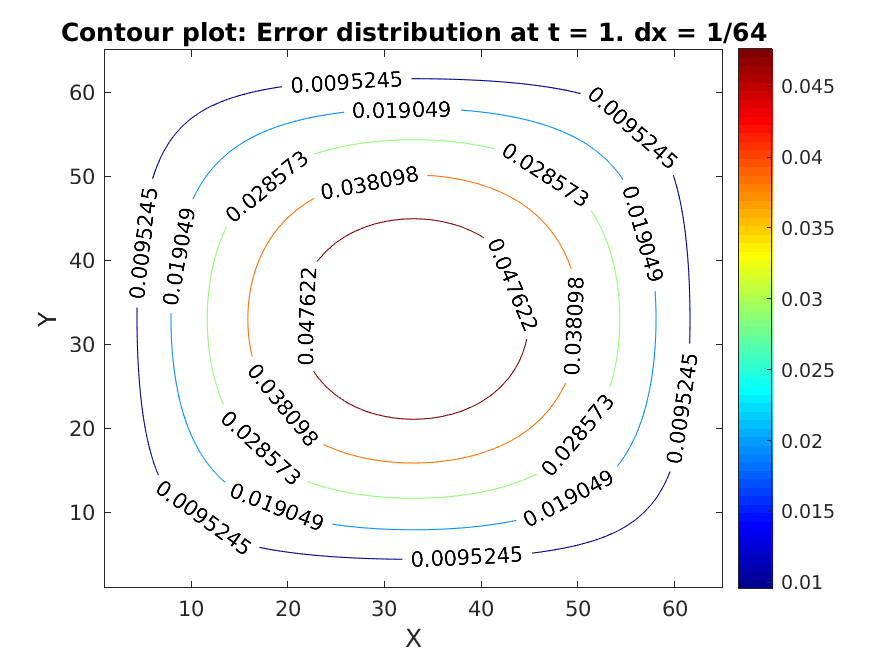
\includegraphics[width=150mm,height= 90mm]{contour_error.png}\hspace*{\fill}
 		\caption{Error distribution 2D plot}
 	\end{figure}
 	\noindent
 	The contour plot gives us a much better detailed view.  We can see that the lowest error is around 0.009, on the outer shell, while the highest error is 0.047. If we try to plot the error with $dx = 1/128$, which is double the previous grid size, then: 
 	\begin{figure}[H]
 		\hfill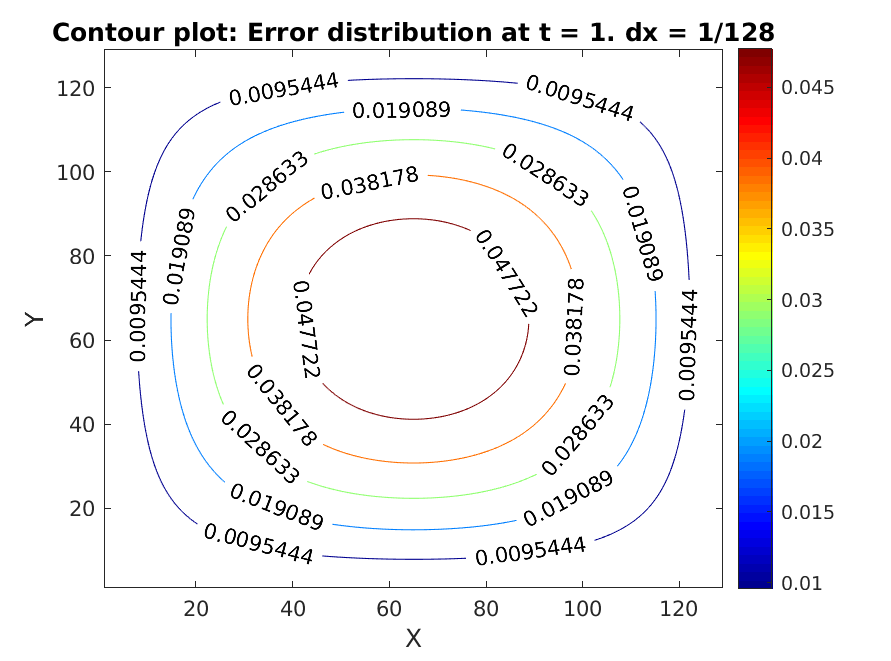
\includegraphics[width=150mm,height= 90mm]{contour128_error.png}\hspace*{\fill}
 		\caption{Error distribution 2D plot at dx = 1/128}
 	\end{figure}
 	 \noindent
 	 Still, the errors are still small, the largest error is around 0.04. Therefore, half dx, which doubles the grid size, does not influence the error very much. If we try to increase the time, let the solution runs till a much later time, then we see this: 
 	 \begin{figure}[H]
 	 	\hfill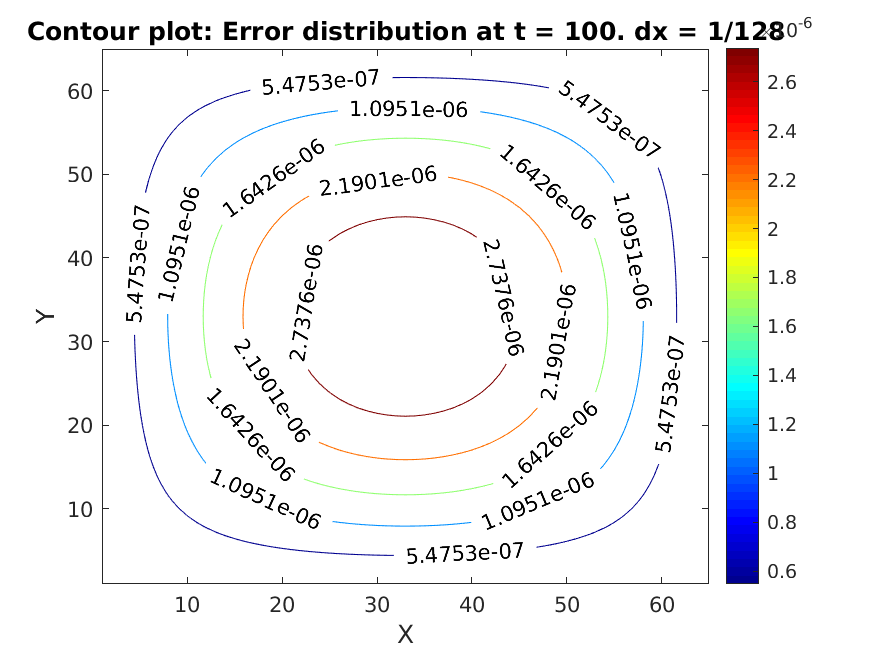
\includegraphics[width=150mm,height= 90mm]{contour100_error.png}\hspace*{\fill}
 	 	\caption{Error distribution 2D plot at dx = 1/128}
 	 \end{figure}
 	 \noindent
 	 The error drastically reduces to order of $10^{-6}$. Therefore, at longer time, the solution does not get smeared or diverged from the analytical solution. In order to show this effectively, as part of the assignment, the following shows the plot between dx and the 2 norm of the error. 
 	 
 	  \begin{figure}[H]
 	 	\hfill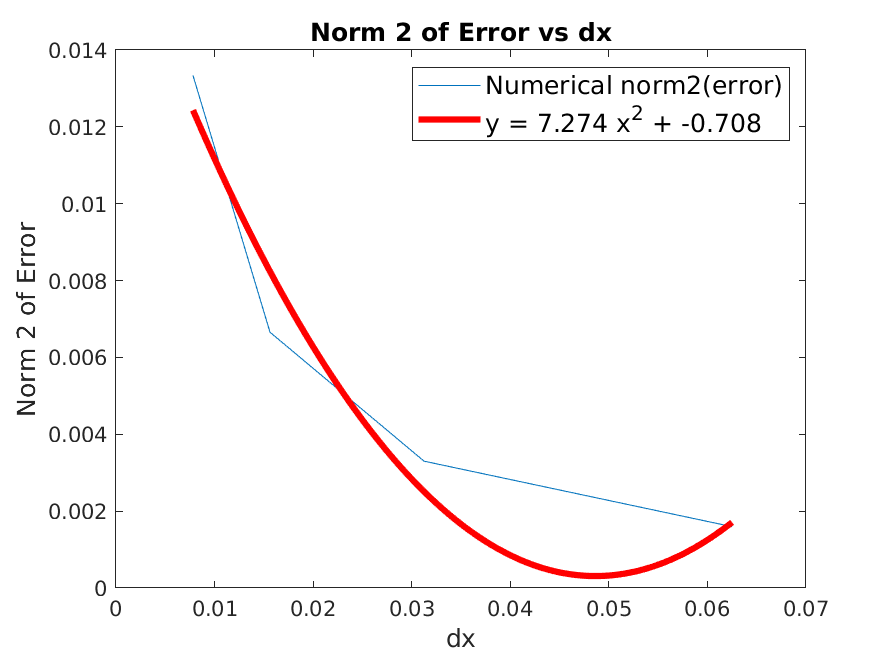
\includegraphics[width=150mm,height= 90mm]{convergence.png}\hspace*{\fill}
 	 	\caption{dx vs Norm 2 of Error}
 	 \end{figure}
 	 \noindent
 	 The figure is to be interpreted as follow: smaller dx means bigger grid size (very coarse grid), bigger dx means smaller grid size (fine grid). Therefore, we can see that as the grid size increases (dx gets smaller), our error goes up. The rate at which this error increases can be modeled by fitting a best fit curve. It turns out that a polynomial of 2nd order ($x^2$) best describes the plot. This makes sense because we use a 2nd order central difference to approximate the derivative, $u_{xx}, u_{yy}$, and this contains a truncation error of O($\Delta x^2$),O($\Delta y^2$). Therefore, our error increases with grid size. The 2-norm in this plot is calculated as follow: 
 	 
 	 \begin{equation}
 	 	||e||_2 = \left(\Delta x \Delta y\sum\limits_{i}^{imax}\sum_{j}^{jmax}|e_{ij}|^2\right)^{1/2}.  	 	
 	 \end{equation}	
 	 
 	 \subsection{Stability Analysis}
 	 Recall Equation 7 and 9, where we derive the ADI scheme at n+1/2 and then n+1,denote $\delta_x^2$ and $\delta_y^2$ to be the second order central difference discretizations, we have the modified equations: 
 	 
 	 \begin{equation}
 	 	(1-\dfrac{1}{2}D_x\delta_x^2)U_{ij}^{n+1/2} = (1-\dfrac{1}{2}D_y\delta_y^2)U_{ij}^{n}  
 	 \end{equation}
 	 
 	 \begin{equation}
 	 	(1-\dfrac{1}{2}D_y\delta_y^2)U_{ij}^{n+1} = (1-\dfrac{1}{2}D_x\delta_x^2)U_{ij}^{n+1/2}  
 	 \end{equation}
 	 We want to apply the Fourier analysis: $F(\vec{u}) = \dfrac{1}{2\pi}\sum\limits_{ij}^{\infty}e^{-Ij\xi-Ij\eta}U_{ij}$. Then for the second order central discretization part, we get: 
 	 
 	 \begin{align*}
 	 	F(\delta_x^2U_{ij}^n) &= F(U_{i+1,j}^n+U_{i-1,j}^n-U_{i,j}^n)\\
 	 	&=\hat{U^n}\left[e^{I\xi}+e^{-I\xi}-2\right]
 	 \end{align*}
 	 Then, apply our two modified equations in similar way. For n to n+1/2: 
 	 
 	 \begin{equation}
 	 	\left(1+2D_xsin^2\left(\dfrac{\xi}{2}\right)\right)\hat{U}^{n+1/2} = \left(1-2D_ysin^2\left(\dfrac{\eta}{2}\right)\right)\hat{U}^{n}
 	 \end{equation}
 	 This yields the amplification factor:
 	 \begin{align*}
 	 	\rho_1(\xi,\eta) &= \dfrac{\hat{U}^{n+1/2}}{\hat{U^n}}\\ &=\dfrac{1-2D_ysin^2\left(\dfrac{\eta}{2}\right)}{1+2D_xsin^2\left(\dfrac{\xi}{2}\right)}
 	 \end{align*}
 	 Likewise, for n+1/2 to n+1: 	 
 	 \begin{equation}
 	 \left(1-2D_xsin^2\left(\dfrac{\xi}{2}\right)\right)\hat{U}^{n+1/2} = \left(1+2D_ysin^2\left(\dfrac{\eta}{2}\right)\right)\hat{U}^{n+1}
 	 \end{equation}
 	 This yields the amplification factor:
 	 \begin{align*}
 	 \rho_2(\xi,\eta) &= \dfrac{\hat{U}^{n+1}}{\hat{U}^{n+1/2}}\\ &=\dfrac{1-2D_xsin^2\left(\dfrac{\xi}{2}\right)}{1+2D_ysin^2\left(\dfrac{\eta}{2}\right)}
 	 \end{align*}
 	 Assuming the overall amplification factor is the multiplication of each individual factor:
 	 \begin{align*}
 	 	\rho(\xi,\eta) &= \rho_1(\xi,\eta)\rho_2(\xi,\eta)\\
 	 	&=\left[\dfrac{1-2D_ysin^2\left(\dfrac{\eta}{2}\right)}{1+2D_xsin^2\left(\dfrac{\xi}{2}\right)}\right]    \left[\dfrac{1-2D_xsin^2\left(\dfrac{\xi}{2}\right)}{1+2D_ysin^2\left(\dfrac{\eta}{2}\right)}\right]\\
 	 \end{align*}
 	 The terms: $2D_xsin^2\left(\dfrac{\xi}{2}\right)$ its similar variations ($\eta$) are always positive due to square. The denominator is always positive because two positive, square parts multiply together. The numerator, we have 1- a positive number, this makes it negative but when multiply by its other counterpart (the other numerator), they become positive. Mathematically, 1 - a square number will be less than 1 + a square number; therefore, the numerator is always less than the denominator: $\rightarrow \rho(\xi,\eta) \leq 1 $. This shows that this ADI scheme is \underline{unconditionally stable}
 	 

	\section{CONCLUSIONS}
	In conclusion, the ADI algorithm solves the parabolic PDE semi-implicitly. First, it solves the X-direction implicitly and Y-direction explicitly. After that, the solution at the half time step is used to solve X-direction explicitly and Y-direction implicitly. The numerical result shows very good similarity with the analytical one. Even if the simulation is left to run until large time such as 100, Figure 13, the numerical solution is still very close to the analytical solution. The error convergence plot shows that as grid size increases (dx gets smaller), the error follows a parabolic path, due to the local truncation error of O($\Delta x^2$). Lastly, the Fourier analysis shows that this ADI scheme is in fact unconditionally stable for arbitrary $D_x,D_y$ or arbitrary grid size and time step. 
	\newpage
	\section{REFERENCE}
	\begin{enumerate}
		\item MTH5315 Numerical Methods for PDE Lecture Notes. Jian,Du. Spring 2018
		\item http://www4.ncsu.edu/~zhilin/TEACHING/MA584/MATLAB/ADI/adi.m. Web. May 5 2018
		\item Tridiagonal Matrix Algorithm. Indian Institute of Space Science and Technology, Thiruvananthapuram. Web. May 5 2018
	\end{enumerate}
	\newpage
	\section{MATLAB CODE}
	\lstinputlisting{max_le_final_MTH5315.m}
	
	
	
\end{document}